\documentclass{beamer}
\usepackage[utf8]{inputenc}
\usetheme{Copenhagen}
%\usepackage[spanish]{babel}
\usepackage{multirow}
%\usepackage{estilo-apuntes}
\usepackage{braids}
\usepackage[]{graphicx}
\usepackage{rotating}
\usepackage{pgf,tikz}
\usepackage{pgfplots}
\usepackage{tikz-cd}
\usepackage{mathtools}
%\usepackage{empheq}
%\usepackage[dvipsnames]{xcolor}
\usepackage{xcolor}

\usetikzlibrary{arrows}
\usetikzlibrary{cd}
\usetikzlibrary{babel}
\pgfplotsset{compat=1.13}
\usetikzlibrary{decorations.shapes}
\pgfkeyssetvalue{/tikz/braid height}{1cm} %no parece hacer nada
\pgfkeyssetvalue{/tikz/braid width}{1cm}
\pgfkeyssetvalue{/tikz/braid start}{(0,0)}
\pgfkeyssetvalue{/tikz/braid colour}{black}

\theoremstyle{definition}

\newtheorem{teorema}{Theorem}
\newtheorem{defi}{Definition}
\newtheorem{prop}[teorema]{Proposition}

\newcommand{\Z}{\mathbb{Z}}
\newcommand{\Q}{\mathbb{Q}}
\newcommand{\C}{\mathbb{C}}
\newcommand{\CC}{\mathcal{C}}
\newcommand{\D}{\mathbb{D}}
\providecommand{\gene}[1]{\langle{#1}\rangle}

\DeclareMathOperator{\im}{im}


\addtobeamertemplate{navigation symbols}{}{%
    \usebeamerfont{footline}%
    \usebeamercolor[fg]{footline}%
    \hspace{1em}%
    %\insertframenumber/\inserttotalframenumber
}
\setbeamercolor{footline}{fg=black}
\setbeamerfont{footline}{series=\bfseries}

\newcommand{\highlight}[1]{%
	\colorbox{red!50}{$\displaystyle#1$}}

\makeatletter
\newcommand*{\encircled}[1]{\relax\ifmmode\mathpalette\@encircled@math{#1}\else\@encircled{#1}\fi}
\newcommand*{\@encircled@math}[2]{\@encircled{$\m@th#1#2$}}
\newcommand*{\@encircled}[1]{%
	\tikz[baseline,anchor=base]{\node[draw,circle,outer sep=0pt,inner sep=.2ex] {#1};}}
\makeatother

\expandafter\def\expandafter\insertshorttitle\expandafter{%
  \insertshorttitle\hfill%
  \insertframenumber\,/\,\inserttotalframenumber}

%-----------------------------------------------------------

\title{What are derived $A_\infty$-structures}
\author{Javier Aguilar Mart\'in}
\institute{University of Kent}
\date{}
 
\begin{document}
\frame{\titlepage}
%\begin{frame}
%
%c¡
%\title[About Beamer] %optional
%{About the Beamer class in presentation making}
% 
%\subtitle{A short story}
% 
%\author[Arthur, Doe] % (optional, for multiple authors)
%{A.~B.~Arthur\inst{1} \and J.~Doe\inst{2}}
% 
%\institute[VFU] % (optional)
%{
%  \inst{1}%
%  Faculty of Physics\\
%  Very Famous University
%  \and
%  \inst{2}%
%  Faculty of Chemistry\\
%  Very Famous University
%}

% 
%\date[VLC 2013] % (optional)
%{Very Large Conference, April 2013}


%\end{frame}
\setbeamercovered{highly dynamic}

\newcounter{saveenumi}
\newcommand{\seti}{\setcounter{saveenumi}{\value{enumi}}}
\newcommand{\conti}{\setcounter{enumi}{\value{saveenumi}}}

\makeatletter
%\newcommand{\xRightarrow}[2][]{\ext@arrow 0359\Rightarrowfill@{#1}{#2}}
\makeatother

\resetcounteronoverlays{saveenumi}
%\AtBeginSection[]{
%\begin{frame}
%\frametitle{Tabla de contenidos}
%\tableofcontents
%\end{frame}
%}

\begin{frame}
INTRO: ASS TO AINFTY TO DAINFTY

ASSOCIATIVITY, NON ASSOCIATIVITY, SOMETHING IN BETWEEN WHERE WE CAN CONTROL THE LACK OF ASSOCIATIVITY

A PATH BETWEEN THE TWO WAYS OF MULTIPLYING 3 ELEMENTS (THIS IS AN  INTUITION FOR HOMOTOPY) TRANSLATE TO ALGEBRA IN TERMS OF BOUNDARY (I WILL HAVE TO CLEAR THAT THE BOUNDARY MAP IS THE BRACKET, NOT D1 ITSELF)

WE CALL M3 THE WHOLE SEGMENT (MULTIPLICATION) AND TAKE BOUNDARRY

PENTAGON (MUST BE FILLED TO HAVE A BOUNDARY) TO PATHS AND HOMOTOPY IN BETWEEN ORIENTATION FOR SIGNS

DIMENSION VS DEGREE

THEN ACTUAL DEFINITIONS, MAYBE SHOW BASIS CASES RECALLING THE PICTURES

UNIQUENESS THEOREMS, FIELD ASSUMPTION, DERIVED
\end{frame}
\section{Introduction}
\begin{frame}
\frametitle{Generalizations of associativity}

Associative algebras $\Rightarrow$ $A_\infty$-algebras $\Rightarrow$ Derived $A_\infty$-algebras
\end{frame}


\begin{frame}
\frametitle{Associativity}
\begin{itemize}
\item $(ab)c=a(bc)$ for all $a,b,c$.
\item[]<2-> Example: \[3\cdot (e\cdot \pi) = (3\cdot e)\cdot \pi = 27\]
\end{itemize}
\end{frame}

\begin{frame}
\frametitle{Non-associativity}
MATRIX MULTIPLICATION

CHECK AS AN EXERCISE
\end{frame}


\section{$A_\infty$-algebras}
\begin{frame}
\frametitle{Measuring the lack of associativity}

IMAGINE PRODUCTS AS POINTS IN THE SPACE
\end{frame}


\begin{frame}
\frametitle{$A_\infty$-algebras}
\begin{defi}
An $A_\infty$-\emph{algebra} $A$ is a module over a ring $k$ equipped with a family of ``multiplications'' $m_n:A^{\otimes n}\to A$ satisfying the relation

$$\sum_{r+s+t=n}(-1)^{rs+t}m_{r+1+t}(1^{\otimes r}\otimes m_s\otimes 1^{\otimes s})=0$$ %we are composing every map with itself
\end{defi}
\end{frame}





\begin{frame}
\frametitle{Some particular cases}
\begin{itemize}
\item<1-> We always have $m_1m_1=0$, so in particular $A$ is a chain complex.%CAN BE DEFINED ON THE CATEGORY OF CHAIN COMPLEX
\item<2-> If $m_i=0$ for $i\neq 2$, the relation becomes $m_2(1\otimes m_2)=m_2(m_2\otimes 1)$, so $A$ is an associative algebra.
\item<3-> If $m_i=0$ for $i\neq 1,2$ we get an extra relation $$m_1m_2=m_2(m_1\otimes 1)+m_2(1\otimes m_1)$$ %MONOID IN CHAIN COMPLEX ANALOGUE TO MONOID IN K-VECT
\item[]<4-> This is the Leibniz rule, and $A$ is a differential graded (dg) algebra.
\end{itemize}
\end{frame}


\begin{frame}
\frametitle{$A_\infty$-algebras are homotopy associative algebras.}
%how do they generalize associative algebras
\begin{itemize}
\item<1-> For $n=3$ we have the relation
\begin{align*}
&m_2(m_2\otimes 1)-m_2(1\otimes m_2)=\\ %the failure of m_2 to be associative
&m_1m_3+m_3(m_1\otimes 1\otimes 1)+m_3(1\otimes m_1\otimes 1)+m_3(1\otimes 1\otimes m_1)
\end{align*}
\item[]<2-> $m_2$ is homotopy associative with homotopy given by $m_3$. %recall that m1 is a differential so on homology this vanishes
\item<3-> The higher relations are a homotopy coherent extension of this fact. %m3 satisfies some relation up to homotopy given by m4 and so on
\end{itemize}
\end{frame}

\section{$A_\infty$-spaces}
\subsection{Loop spaces}
\begin{frame}[fragile]
\frametitle{Where do these algebras come from?} 
%The relation looks random and there could be other ways to generalize associative algebras, but there is a geometric origin
\begin{itemize}
\item<1-> For a pointed space $X$, consider its loop space $\Omega X=\{\gamma:S^1\to X\mid \gamma(1)=*\}$.
\item<2-> $\Omega X$ comes equipped with a ``multiplication'' given by concatenation of loops, but this operation is only associative up to homotopy. 
\end{itemize}

\end{frame}
\begin{frame}
\frametitle{Homotopy-associative product}
\begin{tikzpicture}[line cap=round,line join=round,>=triangle 45,x=1.0cm,y=1.0cm]
\clip(-4.175394430564892,-2.5911383046897085) rectangle (7.490400123879831,3.3976612960713135);
\draw(0.,2.) circle (1.cm);
\draw(0.,-1.) circle (1.cm);
\draw (-3.49428016933844,2.311720973491667) node[anchor=north west] {$(\gamma_1*\gamma_2)*\gamma_3$};
\draw (-3.496796110195476,-0.6773028846978557) node[anchor=north west] {$\gamma_1*(\gamma_2*\gamma_3)$};
\draw (-0.6057688157486263,1.1) node[anchor=north west] {$\gamma_3$};
\draw (0.2964512548334696,0.4) node[anchor=north west] {$\gamma_1$};
\draw (0.7431133461355,2.9675859207922457) node[anchor=north west] {$\gamma_1$};
\draw (-1.3,3.0105934583201526) node[anchor=north west] {$\gamma_2$};
\draw (-1.3,-1.4729423289641315) node[anchor=north west] {$\gamma_2$};
\draw (0.7489686163804383,-1.4729423289641315) node[anchor=north west] {$\gamma_3$};
\draw (2.,2.)-- (3.,1.);
\draw (3.,1.)-- (4.,2.);
\draw (3.,2.)-- (2.514225889472578,1.485774110527422);
\draw (2.,-1.)-- (3.,-2.);
\draw (3.,-2.)-- (4.,-1.);
\draw (3.,-1.)-- (3.481998691455241,-1.518001308544759);
\draw (1.7811495170502019,2.6342775049509677) node[anchor=north west] {$\gamma_1$};
\draw (2.8240823021019423,2.623525620568991) node[anchor=north west] {$\gamma_2$};
\draw (3.7487443589519387,2.5912699674230613) node[anchor=north west] {$\gamma_3$};
\draw (1.7811495170502019,-0.4085057751484382) node[anchor=north west] {$\gamma_1$};
\draw (2.8133304177199654,-0.4085057751484382) node[anchor=north west] {$\gamma_2$};
\draw (3.813255665243799,-0.4300095439123916) node[anchor=north west] {$\gamma_3$};
\draw [->] (1.,2.) -- (0.9776684310102762,2.2101533701987783);
\draw [->] (0.,3.) -- (-0.2228209821222102,2.9748593795651215);
\draw [->] (-1.,2.) -- (-0.9818938166599703,1.8105678675490438);
\draw [->] (1.,-1.) -- (0.9832067635335799,-0.8175049037869153);
\draw [->] (-1.,-1.) -- (-0.9827773938908082,-1.1847933820708718);
\draw [->] (0.,-2.) -- (0.1987984337916885,-1.9800403985152712);
\end{tikzpicture}
\end{frame}
\begin{frame}
\frametitle{Homotopy coherence}
\definecolor{dcrutc}{rgb}{0.39215686274509803,0.39215686274509803,0.39215686274509803}
\begin{tikzpicture}[line cap=round,line join=round,>=triangle 45,x=1.0cm,y=1.0cm]
\clip(-3.0601652892561972,-1.781126972201351) rectangle (5.063801652892563,3.6734184823441027);
\fill[color=dcrutc,fill=dcrutc,fill opacity=0.10000000149011612] (2.5,2.5) -- (0.5,2.5) -- (-0.1180339887498949,0.5978869674096935) -- (1.5,-0.5776835371752531) -- (3.118033988749895,0.5978869674096927) -- cycle;
\draw (2.5,2.5)-- (0.5,2.5);
\draw (0.5,2.5)-- (-0.1180339887498949,0.5978869674096935);
\draw (-0.1180339887498949,0.5978869674096935)-- (1.5,-0.5776835371752531);
\draw (1.5,-0.5776835371752531)-- (3.118033988749895,0.5978869674096927);
\draw (3.118033988749895,0.5978869674096927)-- (2.5,2.5);
\draw (-0.4298121712997737,3.113688955672426)-- (0.16372652141247268,2.6629000751314793);
\draw (0.16372652141247268,2.6629000751314793)-- (0.6445679939894825,3.196333583771599);
\draw (-0.24422955190381973,2.9727401308147394)-- (-0.1367993989481584,3.113688955672426);
\draw (-0.031385527253731726,2.8110864412070775)-- (0.17123966942148847,3.10617580766341);
\draw (-1.2938241923365879,0.8973102930127725)-- (-0.6627197595792627,0.4314951164537945);
\draw (-0.6627197595792627,0.4314951164537945)-- (-0.16685199098422132,0.9649286250939145);
\draw (-0.8706947249429613,0.5850004480317625)-- (-0.5049436513899312,0.9799549211119465);
\draw (-0.6957015377932548,0.7739659686300595)-- (-0.9106536438767833,0.9799549211119465);
\draw (0.869962434259956,-0.8908189331329814)-- (1.516093163035313,-1.3791735537190069);
\draw (1.516093163035313,-1.3791735537190069)-- (2.0645529676934644,-0.8532531930879026);
\draw (1.699788860636136,-1.203026994375752)-- (1.1930277986476345,-0.838226897069871);
\draw (1.4723143911047147,-1.0392758405399645)-- (1.6888955672426758,-0.838226897069871);
\draw (3.2516303531179576,0.8522314049586783)-- (3.8151164537941407,0.2737190082644637);
\draw (3.8151164537941407,0.2737190082644637)-- (4.416168294515403,0.8221788129226153);
\draw (4.236244854403876,0.6579986738208468)-- (4.055537190082646,0.8372051089406468);
\draw (4.037275969199595,0.47643956607194105)-- (3.634800901577762,0.86725770097671);
\draw (2.2373553719008274,3.1437415477084896)-- (2.7783020285499633,2.5802554470323065);
\draw (2.7783020285499633,2.5802554470323065)-- (3.37184072126221,3.1136889556724268);
\draw (2.4140676158297834,2.959666293615827)-- (2.590473328324569,3.136228399699474);
\draw (3.189075837510895,2.949431908250359)-- (3.0112096168294524,3.1212021036814424);
\draw [->] (0.8624492862509402,2.880781367392938) -- (1.9894214876033067,2.8657550713749065);
\draw [->] (3.168985725018784,2.5351765589782125) -- (3.612261457550715,1.1903230653643886);
\draw [->] (-0.12928625093914242,2.647873779113449) -- (-0.6101277235161522,1.3180465815176567);
\draw [->] (-0.29457550713748953,0.12345604808414862) -- (0.6370548459804668,-0.78563486100676);
\draw [->] (2.395131480090159,-0.755582268970697) -- (3.37184072126221,0.1535086401202117);
\end{tikzpicture}
%filling the pentagon means finding a homotopy between the two paths of homotopies
\end{frame}

\subsection{$A_\infty$-spaces}
\begin{frame}
A space with such a homotopy coherent multiplication is called an $A_\infty$-space.\pause
\begin{theorem}[P. May]%homology of iterated loop spaces
Let $Z$ be an $A_\infty$-space (for instance $Z=\Omega X$), then the singular chain complex $C_*(Z)$ is an $A_\infty$-algebra.
\end{theorem}
%The A-infty-structre on the space induce an A_infty-algebra
\end{frame}

\section{Hochschild Complex}
\begin{frame}
%we are now going to discuss another way to obtain an A_\infty algebra, this time from an already existing A_\infty algebra
\begin{defi}
	The \emph{Hochschild complex} of a $k$-module $A$ is given by the modules $C^m(A;A)=\hom_k(A^{\otimes m}, A)$, where $C^0(A;A)=A$.% and the differential
	% \begin{align*}
%	 \delta_m f(a_1\otimes\cdots\otimes a_{m+1})&=a_1f(a_2\otimes\cdots\otimes a_{m+1})\\
%	  +\sum_{i=1}^m(-1)^if(a_1\otimes\cdots&\otimes a_{i-1}\otimes a_ia_{i+1}\otimes a_{i+1}\otimes\cdots a_{m+1})\\
%	 & +(-1)^{m+1}f(a_1\otimes\cdots\otimes a_m)a_{m+1}
	 %\end{align*}
	 \end{defi}\pause
	 %explain that the diferential is just multiplying consecutive elements
	 An element $f\in C^n(A;A)$ is a map $f:A^{\otimes n}\to A$, so we represent it as
	 
	\begin{tikzpicture}[line cap=round,line join=round,>=triangle 45,x=1.0cm,y=1.0cm]
	\clip(-2.8466666666666676,-1) rectangle (11.486666666666668,3);
	\draw[line width=1.pt] (0.,0.) -- (0.,1.38) -- (2.406666666666667,1.38) -- (2.406666666666667,0.) -- cycle;
	\draw [line width=1.pt] (0.,0.)-- (0.,1.38);
	\draw [line width=1.pt] (0.,1.38)-- (2.406666666666667,1.38);
	\draw [line width=1.pt] (2.406666666666667,1.38)-- (2.406666666666667,0.);
	\draw [line width=1.pt] (2.406666666666667,0.)-- (0.,0.);
	\draw [line width=.pt] (1.2033333333333336,0.)-- (1.2033333333333336,-0.606666666666666);
	\draw [line width=1.pt] (1.2033333333333336,1.38)-- (1.2033333333333336,2.3933333333333344);
	\draw [line width=1.pt] (0.7666666666666668,2.3933333333333344)-- (0.7666666666666668,1.38);
	\draw [line width=1.pt] (0.3933333333333334,2.3933333333333344)-- (0.38,1.38);
	\draw [line width=1.pt] (1.606666666666667,2.3933333333333344)-- (1.606666666666667,1.38);
	\draw [line width=1.pt] (1.9933333333333336,2.3933333333333344)-- (1.9933333333333336,1.38);
	\draw (1.,0.9933333333333343) node[anchor=north west] {$f$};
	\end{tikzpicture}

\end{frame}
\subsection{Braces}
\begin{frame}


	\frametitle{Brace algebra on $C^*(A;A)$}
	
	\begin{itemize}
		\item Let $f,g_1,\dots, g_n\in C^*(A;A)$. Then the \emph{brace} $f\{g_1,\dots, g_n\}$ is given by %this comes with signs that we don't include
		
		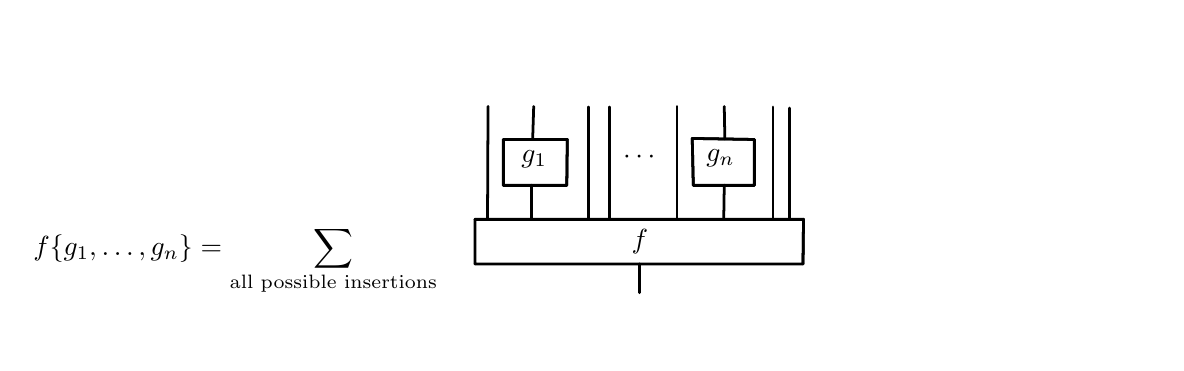
\begin{tikzpicture}[line cap=round,line join=round,>=triangle 45,x=1.0cm,y=1.0cm]
		\clip(-2.8466666666666676,-1) rectangle (11.486666666666668,3);
		\draw[line width=1.pt] (2.833333333333334,0.) -- (2.833333333333334,0.5666666666666675) -- (7.006666666666668,0.5666666666666675) -- (7.,0.) -- cycle;
		\draw[line width=1.pt] (3.193333333333334,1.) -- (4.,1.) -- (4.006666666666668,1.58) -- (3.193333333333334,1.58) -- cycle;
		\draw[line width=1.pt] (6.,1.) -- (6.38,1.) -- (6.38,1.58) -- (5.593333333333335,1.5933333333333344) -- (5.606666666666667,1.) -- cycle;
		\draw (-2.9,0.6) node[anchor=north west] {$f\{g_1,\dots, g_n\}=\displaystyle{\sum_{\text{all possible insertions}}}$};
		\draw [line width=1.pt] (2.833333333333334,0.)-- (2.833333333333334,0.5666666666666675);
		\draw [line width=1.pt] (2.833333333333334,0.5666666666666675)-- (7.006666666666668,0.5666666666666675);
		\draw [line width=1.pt] (7.006666666666668,0.5666666666666675)-- (7.,0.);
		\draw [line width=1.pt] (7.,0.)-- (2.833333333333334,0.);
		\draw [line width=1.pt] (4.92,0.)-- (4.92,-0.36666666666666614);
		\draw [line width=1.pt] (2.993333333333334,0.5666666666666675)-- (3.,2.);
		\draw [line width=1.pt] (3.553333333333334,0.5666666666666675)-- (3.553333333333334,1.);
		\draw [line width=1.pt] (4.273333333333334,0.5666666666666675)-- (4.273333333333334,1.9933333333333345);
		\draw [line width=1.pt] (4.54,0.5666666666666675)-- (4.54,1.9933333333333345);
		\draw [line width=1.pt] (5.993333333333334,0.5666666666666675)-- (6.,1.);
		\draw [line width=1.pt] (6.62,0.5666666666666675)-- (6.62,1.9933333333333345);
		\draw [line width=1.pt] (6.833333333333335,0.5666666666666675)-- (6.833333333333335,1.98);
		\draw [line width=1.pt] (3.193333333333334,1.)-- (4.,1.);
		\draw [line width=1.pt] (4.,1.)-- (4.006666666666668,1.58);
		\draw [line width=1.pt] (4.006666666666668,1.58)-- (3.193333333333334,1.58);
		\draw [line width=1.pt] (3.193333333333334,1.58)-- (3.193333333333334,1.);
		\draw [line width=1.pt] (6.,1.)-- (6.38,1.);
		\draw [line width=1.pt] (6.38,1.)-- (6.38,1.58);
		\draw [line width=1.pt] (6.38,1.58)-- (5.593333333333335,1.5933333333333344);
		\draw [line width=1.pt] (5.593333333333335,1.5933333333333344)-- (5.606666666666667,1.);
		\draw [line width=1.pt] (5.606666666666667,1.)-- (6.,1.);
		\draw [line width=1.pt] (3.5666666666666673,1.58)-- (3.58,2.);
		\draw [line width=1.pt] (6.007451656136321,1.586314378709553)-- (6.,2.);
		\draw [line width=1.pt] (5.4,0.5666666666666675)-- (5.4,2.);
		\draw (3.3,1.5666666666666678) node[anchor=north west] {$g_1$};
		\draw (5.65,1.58) node[anchor=north west] {$g_n$};
		\draw (4.7,0.5666666666666675) node[anchor=north west] {$f$};
		\draw (4.59,1.5533333333333343) node[anchor=north west] {$\cdots$};
		\end{tikzpicture}
		\item<2-> $f\{\}=f$. %when the arity is lower than n the brace is defined to be 0
	\end{itemize}
\end{frame}

\begin{frame}
\begin{itemize}
\item<1-> Let $A$ be an $A_\infty$-algebra and let $m=m_1+m_2+\cdots$.
\item<2-> Define maps $M_i:C^*(A;A)^{\otimes n}\to C^*(A;A)$ by
\begin{align*}
M_1(f)\coloneqq &m\{f\}-f\{m\}\\ %this is indeed a Lie bracket
M_n(f_1,\dots, f_n)\coloneqq &m\{f_1,\dots, f_n\} & n>1
\end{align*}
\end{itemize}
\end{frame}





\begin{frame}
\begin{theorem}[Getzler]
The maps $M_i$ define an $A_\infty$-algebra structure on the Hochschild complex $C^*(A;A)$.
\end{theorem}
\begin{itemize}
\item<2-> In particular, when $A$ is associative, $C^*(A;A)$ is associative and $M_2$ coincides with the usual cup product 
\[f\smile g(a_1,\dots,a_{n+m})=f(a_1,\dots, a_n)g(a_{n+1},\dots, a_{n+m}).\]
\item<3-> In this case the differential $M_1$ takes the form
 \begin{align*}
	 M_1 f(a_1\otimes\cdots\otimes a_{m+1})&=a_1f(a_2\otimes\cdots\otimes a_{m+1})\\
	  +\sum_{i=1}^m(-1)^if(a_1\otimes\cdots&\otimes a_{i-1}\otimes a_ia_{i+1}\otimes a_{i+1}\otimes\cdots a_{m+1})\\
	 & +(-1)^{m+1}f(a_1\otimes\cdots\otimes a_m)a_{m+1}
	 \end{align*}

\end{itemize}
\end{frame}
\begin{frame}
\frametitle{$A_\infty$-equation in terms of a bracket}
\begin{itemize}
\item[]<1->\begin{block}{Remark}
The operation $[f,g]=f\{g\}-g\{f\}$ is a Lie bracket. %there is a richer structure
\end{block}
\item<2-> The equation $m_1m_1=0$ is equivalent to $[m_1,m_1]=0$.
\item<3-> The Leibniz rule is equivalent is equivalent to $[m_1,m_2]=0$.
\item<4-> The homotopy associativity equation (case $n=3$) is equivalent to $m_2\{m_2\}=[m_1,m_3]$. In particular associativity is equivalent to $[m_2,m_2]=0$. %it is equivalent to the brace=0 but the bracket is obtained from the brace %not only zero in the homology of A as a chain complex but also in the hochschild cohomology with respect to m1 that I'll mention later
\item<5-> In general, an $A_\infty$-algebra is equivalent to the condition $[m,m]=0$ where $m=m_1+m_2+\cdots$.
\end{itemize}

\end{frame}
\begin{frame}
%there is a relation between the original structurer and the induced one
\begin{theorem}[Gerstenhaber-Voronov]
The map $\Phi:A\to C^*(A;A)$ defined by \[\Phi(x)=\sum_{n\geq 0} x\{x_1,\dots, x_n\}\]
is a map of $A_\infty$-algebras, i.e. it satisfies 
\[\Phi(M_n)=M_n(\Phi^{\otimes n})\]
for all $n$.

\end{theorem}
\end{frame}
\section{Cohomology}
\begin{frame}
\frametitle{Hochschild cohomology}
\begin{itemize}
\item<1-> Since $M_1$ is a differential, we can define the  cohomology of $C^*(A;A)$ with respect to $M_1$. 
\item<2-> We call this cohomology $H^*(A;A)$ the \emph{Hochschild cohomology} of $A$.
\item<3-> What kind of structure does this cohomology have?
\end{itemize}
\end{frame}

\begin{frame}
\begin{itemize}

\item<1-> If $A$ is an associative algebra, $H^*(A;A)$ is a \emph{Gerstenhaber algebra}: it has an associative and commutative product given by the cup product and a Lie bracket given by the braces as before, such that the bracket is a derivation of the product.
\item<2-> A description for the general case is still unknown.
\end{itemize}



\end{frame}



\end{document}
